\chapter{Order From Understanding Disorder}

This chapter follows J. Krishnamurti's fifth San Diego conversation with Allan W. Anderson on order, disorder, thought, measurement, comparison, and observation. There are no retained blackboard frames for this lecture, so the mathematical form below is deliberately modest: we use equations and diagrams only as compact notation for the spoken inquiry. The primary movement is not from theorem to theorem, but from a false idea of order to a precise question: can order appear without being imposed by a mind that is itself disorderly?

\section{The Question Of Order In Freedom}

The conversation begins by returning to a previous field of inquiry: freedom, responsibility, and relationship. Before going further, Krishnamurti proposes that they talk over order. The first formulation is already restrictive:

\begin{equation}
\text{order in freedom} \neq \text{order by control}.
\end{equation}

That distinction governs the whole chapter. If order is simply control, discipline, conformity, or obedience, then freedom has already disappeared. But if order belongs to freedom, then we have to ask what order is without importing the usual machinery of command.

The conversation does not begin with an ideal definition. It begins with the observation of disorder. Krishnamurti points to disorder outwardly and inwardly: in countries, religions, governments, business, family life, morality, sex, and personal relationship. The survey matters because it prevents us from treating disorder as a private mood. Disorder is not only an individual disturbance, nor only a social malfunction. The question is whether the outward disorder and the inward disorder are two separate facts or one movement.

Anderson introduces the first structural clue. Perhaps what we call order is repeatedly superimposed on an existing situation. The imposed order does not heal the disorder; it creates a new situation, which then demands another imposed order. Written schematically, the pattern is

\begin{equation}
\text{disorder} + \text{imposed ideal of order}
\longrightarrow
\text{new disorder}.
\end{equation}

This is not a formal law. It is a compact way of preserving the lecture's first diagnosis: a disordered mind cannot be made orderly by an external pattern imposed upon it. The imposition becomes part of the disorder.

\section{Imposed Order As Disorder}

Krishnamurti tests the ordinary meanings of order one by one. Is order military discipline? Is it conformity? Is it obedience? Is it imitation? Is it acceptance of authority? The repeated form of the question is important. He is not merely making a list of bad social habits. He is asking whether the very instruments by which we usually seek order are among the causes of disorder.

The conceptual distinction can be written as

\begin{equation}
\text{order} \neq
\text{conformity},\quad
\text{imitation},\quad
\text{obedience},\quad
\text{suppression}.
\end{equation}

The reason is not that conformity is unpleasant, or that obedience is unfashionable. The reason is sharper. If I conform to an order imposed from outside or from an idea, I create a division between what I am and what I think I should be. That division carries conflict. Conflict is already disorder.

\begin{proposition}
In the logic of this conversation, imposed order is not the opposite of disorder. It is one of disorder's forms.
\end{proposition}

\begin{proof}
The imposed order begins from an ideal, an authority, or a pattern. The mind that receives the pattern is already fragmented. The pattern therefore enters as pressure: conformity, suppression, imitation, or resistance. Pressure produces conflict, and conflict is disorder. Thus the imposed order does not end disorder; it extends it.
\end{proof}

The same applies to authority. Whether the authority is political, religious, pedagogical, or psychological, it commonly appears as someone saying: I know, and you do not know. Krishnamurti treats that relation as one of the factors that has produced disorder. The problem is not merely bad authority; it is the structure of dependence and division that authority can create.

\section{Studying The Movement Of Disorder}

The first turning point comes when Krishnamurti says that order comes from understanding disorder. We must not first seek order and then impose it. We must understand the nature, structure, and movement of disorder.

\begin{equation}
\text{understanding disorder}
\longrightarrow
\text{order}.
\end{equation}

The arrow should be read cautiously. It does not mean a method, a technique, or a sequence of exercises. It means that order is not separately manufactured. It appears in the understanding of disorder.

\subsection{Question \& Answer}

\paragraph{Question.}
Anderson raises the natural objection. If disorder is disorder, if by its own condition it has no ordering principle, how can it be studied? Are we being asked to study something that is intrinsically unstudiable?

\paragraph{Answer.}
Krishnamurti's answer shifts the object of study. We are not studying disorder as a dead category. We are studying the movement of disorder. Once the word ``movement'' enters, the inquiry becomes concrete. Disorder acts. It spreads. It corrupts. It destroys. It is not an abstract label but a living process.

We can record the shift as

\begin{align}
\text{disorder as concept} &\quad \text{appears unstudiable},\\
\text{disorder as movement} &\quad \text{can be observed}.
\end{align}

The image of sitting on the bank of a river belongs here. One cannot alter the water by staring at it, but one can watch its movement. In the same way, the movement of disorder is not to be controlled first and understood later. It must be seen as it moves.

\section{Thought, Fragmentation, And Opposites}

Krishnamurti next asks for the factor of disorder. His answer is not social first, but structural: thought is fragmentary. Thought is described as the response of memory, experience, and the past. Therefore thought divides.

The chain is compactly represented as

\begin{equation}
\text{memory/past}
\longrightarrow
\text{thought}
\longrightarrow
\text{fragmentation}
\longrightarrow
\text{division}
\longrightarrow
\text{conflict}
\longrightarrow
\text{disorder}.
\end{equation}

This equation-like line must not be read as mechanical psychology. It is a map of the conversation's order. Thought divides me from not-me, my country from your country, my belief from your belief, my religion from your religion. The very movement of thought is divisive when it operates from the past as a fragment.

The dialogue then sharpens the distinction between difference and division. There are descriptive distinctions: man and woman, black and white, this object and that object. But descriptive distinction is not the same as psychological division. Division begins when thought turns distinction into opposition, and opposition into conflict.

Krishnamurti's example is violence. Is there an opposite to violence, or is there only violence? He says thought creates the opposite, non-violence, and then conflict begins between the fact and the abstraction.

\begin{align}
\text{violence} & = \text{what is},\\
\text{non-violence} & = \text{abstraction from what is},\\
\text{fact} + \text{abstraction} & \longrightarrow \text{conflict}.
\end{align}

Anderson confirms the same structure through another pair: vice and virtue. Virtue is not simply the opposite of vice. If virtue is treated as the opposite of vice, it remains inside the conceptual structure of opposition. The chapter should preserve this subtlety because it is one of the lecture's central distinctions: the false opposite is not liberation from the fact; it is thought's continuation of conflict.

\section{Measurement, Comparison, And The Immeasurable}

The conversation then pivots to measurement. Krishnamurti links Western civilisation with measurement, technology, commercialism, and consumerism. He then contrasts this with Indian religious language about the immeasurable: measurement must come to an end if the immeasurable is to be found. But the difficulty is that thought then tries to control thought in order to reach the immeasurable.

The point can be written as a small derivation.

\begin{enumerate}
\item The mind says that measurement must end.
\item The mind proposes to end measurement by controlling thought.
\item The controller of thought is another movement of thought.
\item Therefore the attempt to end measurement by control remains within measurement.
\end{enumerate}

In notation:

\begin{equation}
\text{controller of thought}
=
\text{fragment of thought}.
\end{equation}

Therefore,

\begin{equation}
\text{thought controlling thought}
\longrightarrow
\text{measurement using measurement}.
\end{equation}

This is the lecture's most precise critique of method. A method that promises to end the movement of thought may itself be another fragment of thought. It can polish the structure of measurement without going beyond it.

Krishnamurti then gives the most direct equation-like statement in the lecture:

\begin{definition}
In this conversation, measurement means comparison:
\begin{equation}
\text{measurement}=\text{comparison}.
\end{equation}
\end{definition}

Comparison appears in education, religion, status, success, intelligence, dullness, hierarchy, and spiritual becoming. One person is compared with another; one state is compared with another; the present self is compared with the ideal self. The movement of comparison becomes the movement of becoming: more, less, higher, lower, nearer, farther.

The chapter can preserve Anderson's mathematical aside without turning it into number theory. He observes that mathematics has an order in which one integer does not become another by becoming larger. Two stops at two:

\begin{equation}
2.5 \neq 2.
\end{equation}

His point is not about decimal notation. It is about the clarity of order. If we are speaking of the integer two, then ``two and a half'' is no longer two. The aside helps the reader see why comparison and gradual becoming may be the wrong model for the kind of order under discussion. Order is not the endless enlargement of disorder into something better. It is a different movement.

\begin{figure}
\centering
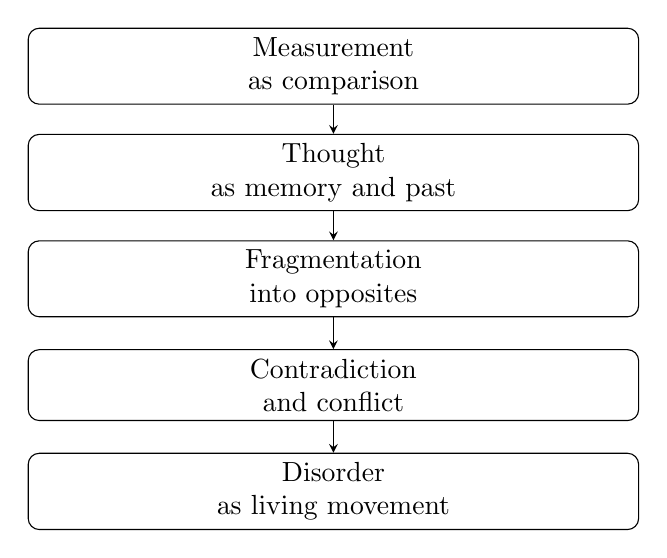
\begin{tikzpicture}[>=stealth]
\node[draw, rounded corners, align=center, text width=0.62\linewidth] (a) at (0,0) {Measurement\\as comparison};
\node[draw, rounded corners, align=center, text width=0.62\linewidth] (b) at (0,-1.35) {Thought\\as memory and past};
\node[draw, rounded corners, align=center, text width=0.62\linewidth] (c) at (0,-2.70) {Fragmentation\\into opposites};
\node[draw, rounded corners, align=center, text width=0.62\linewidth] (d) at (0,-4.05) {Contradiction\\and conflict};
\node[draw, rounded corners, align=center, text width=0.62\linewidth] (e) at (0,-5.40) {Disorder\\as living movement};
\draw[->] (a) -- (b);
\draw[->] (b) -- (c);
\draw[->] (c) -- (d);
\draw[->] (d) -- (e);
\end{tikzpicture}

A transcript-backed conceptual map of the lecture's middle movement. The arrows mark the order of inquiry, not a mechanical theory.
\end{figure}

\section{The Fact Without Comparison}

The lecture then turns from comparison to the possibility of looking without comparison. Anderson recalls seeing a globule of dew on a lotus leaf in Bangkok. At first he asks questions: where is the base, how can it be stable, why does it not roll off? Then the questioning exhausts itself, and he simply looks. The importance of the story is not decorative. It gives the lecture a concrete instance of fact without conceptual interference.

Krishnamurti receives the example as pointing to what he means by remaining with the fact. The globule on the leaf is the fact. It is the act. It is what is done. Nothing has to be compared with it in order for it to be seen.

From this arises the educational question: can one educate a student to live without comparison? The ordinary school and university system is comparative almost from the beginning. One child is dull, another clever; one succeeds, another fails. Krishnamurti reverses the premise. I know that I am dull only through comparison. If I do not compare, I do not know what I am in that way. Then I begin there.

The conceptual contrast can be made in a small table.

\begin{table}
\centering
\begin{tabular}{p{0.43\linewidth} p{0.43\linewidth}}
\textbf{Comparison} & \textbf{Non-comparative looking}\\
Measures one state against another & Begins with the fact as it is\\
Creates more and less & Does not move by hierarchy\\
Sustains anxiety and competition & Ends that particular conflict\\
Asks what I should become & Asks what is actually present\\
\end{tabular}

A compact contrast drawn from the conversation on measurement and comparison.
\end{table}

The phrase ``totally ordered'' enters here. Anderson notices that Krishnamurti often uses total and absolute. The point is not absolutism as dogma. It is that there is no bridge from total disorder to total order by gradual comparison. If the movement is comparative, it remains within measurement.

\section{Can The Disorderly Mind Observe Disorder?}

The most difficult question now appears. We have said that disorder must be understood. But the mind that is to understand disorder is itself disorderly. Can such a mind observe the movement of disorder?

\subsection{Question \& Answer}

\paragraph{Question.}
Can the mind, already in a state of disorder, observe disorder without introducing an observer who imagines himself orderly?

\paragraph{Answer.}
Krishnamurti says that this imagined observer is itself part of disorder. The observer who says, ``I am orderly and I will put order into disorder,'' is the past, the divider, the maker of opposition. Therefore the observer is not outside the observed disorder.

The central proposition is

\begin{equation}
\text{observer}=\text{observed}.
\end{equation}

And near the end of the same movement:

\begin{equation}
\text{perceiver}=\text{perceived}.
\end{equation}

Again, these are not algebraic identities. They are precise statements about the structure of division. The observer who claims to stand apart from disorder is made of the same movement: memory, past, measurement, comparison, fragmentation. Where there is division, there is conflict; where there is conflict, there is disorder. So the observer cannot be the agent that brings order.

\begin{proposition}
A mind cannot bring order to disorder by introducing an observer who is imagined to be separate from disorder.
\end{proposition}

\begin{proof}
The observer is constructed by thought as an opposite to what is observed. Thought is memory and past, and its movement is fragmentary. A fragment that stands apart from another fragment creates division. Division produces conflict. Therefore the observer introduced as an ordering agent is itself a factor of disorder. It cannot bring about order.
\end{proof}

The alternative is stated negatively and simply: observe without the observer, perceive without the perceiver. This is not a technique. If it becomes a technique, it has already acquired a controller, and the controller is another fragment of thought.

\begin{figure}
\centering
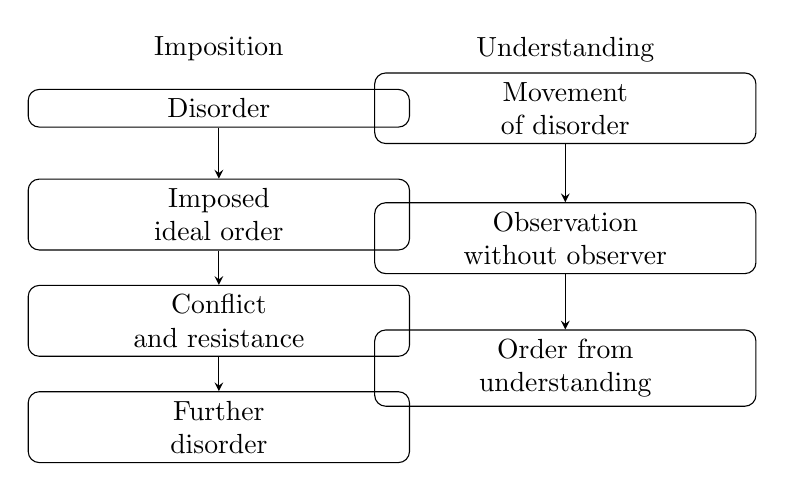
\begin{tikzpicture}[>=stealth]
\node[draw, rounded corners, align=center, text width=0.38\linewidth] (d1) at (-2.2,0) {Disorder};
\node[draw, rounded corners, align=center, text width=0.38\linewidth] (i1) at (-2.2,-1.35) {Imposed\\ideal order};
\node[draw, rounded corners, align=center, text width=0.38\linewidth] (c1) at (-2.2,-2.70) {Conflict\\and resistance};
\node[draw, rounded corners, align=center, text width=0.38\linewidth] (fd1) at (-2.2,-4.05) {Further\\disorder};
\draw[->] (d1) -- (i1);
\draw[->] (i1) -- (c1);
\draw[->] (c1) -- (fd1);

\node[draw, rounded corners, align=center, text width=0.38\linewidth] (d2) at (2.2,0) {Movement\\of disorder};
\node[draw, rounded corners, align=center, text width=0.38\linewidth] (o2) at (2.2,-1.65) {Observation\\without observer};
\node[draw, rounded corners, align=center, text width=0.38\linewidth] (or2) at (2.2,-3.30) {Order from\\understanding};
\draw[->] (d2) -- (o2);
\draw[->] (o2) -- (or2);

\node[align=center] at (-2.2,0.75) {Imposition};
\node[align=center] at (2.2,0.75) {Understanding};
\end{tikzpicture}

Two transcript-backed paths: imposed order extends disorder, while understanding begins with observation of disorder's movement.
\end{figure}

This is also where Krishnamurti returns the disorder from ``out there'' to ``in here.'' Governments, wars, divisions among nations, religions, and ideologies are not treated as external accidents. They are expressions of the same fragmented human mind. This is why political and religious attempts to impose order are called palliatives. They repeat the same structure: a divided mind tries to solve division by means of division.

\section{Order, Virtue, Conduct, And Attention}

After the observer discussion, Krishnamurti recaps the central thesis: order comes only with the understanding of disorder. In that understanding there is no superimposition, no suppression, no conflict. Order is then described as a different kind of movement.

He identifies that order with virtue. Here virtue is not an opposite to vice and not a theory of moral improvement. Virtue is conduct. Anderson adds that in the I Ching the hexagram called conduct is also translated as treading, which suggests movement. Krishnamurti accepts the point. Conduct is not a fixed moral pose. It is the movement of a life in order.

We can summarize the final movement as

\begin{equation}
\text{seeing the movement of disorder}
\longrightarrow
\text{order}
\longrightarrow
\text{virtue as conduct}.
\end{equation}

But the same caution applies. If this line is taken as a procedure, it has already been falsified. The seeing is not the result of a controller. It is not a method for stilling the mind. Anderson explicitly notes that any technique for stilling the mind requires a stiller, and that stiller is another form of the division already exposed.

The lecture ends by returning to attention. Anderson says that he begins to understand the emphasis on staying totally attentive to this. But then another phenomenon appears: as one begins to think one is leaning into the inquiry, fear arises. The next conversation will take up fear. This ending should remain open. Order has been clarified, but the inquiry has not closed; it has reached the threshold of fear.

\section{Summary}

This conversation gives order a precise negative and positive structure. Negatively, order is not conformity, not imitation, not obedience, not suppression, not authority, and not an ideal imposed on disorder. Positively, order comes with the understanding of the movement of disorder.

The movement of disorder is traced through thought. Thought is the response of memory and the past; as such it is fragmentary. Fragmentation becomes division, division becomes contradiction, and contradiction becomes conflict. Measurement, in the sense of comparison, is one of the central ways this fragmentation continues. It appears in education, hierarchy, religion, self-image, and the desire to become something other than what is.

The decisive point is the observer. The mind that tries to observe disorder by standing apart from it invents an orderly observer. But that observer is itself part of disorder, because it is the past and the maker of division. Thus the observer is the observed. To see disorder without the observer is the new factor in the conversation. From that seeing, Krishnamurti says, order is not imposed; it flowers as virtue, conduct, responsibility, and attention.